\documentclass{beamer}

\mode<presentation>
{%
	\usetheme{Warsaw}
	\setbeamercovered{invisible}
}
\setbeamertemplate{caption}[numbered] 
\setbeamerfont{caption}{size=\scriptsize}

\usepackage[spanish]{babel}
\usepackage[utf8]{inputenc}
\usepackage{url}
\usepackage{subfig}

\title{Managing the Development of Large Software Systems}

\author[Pipe \& Filter]{%
	{\Large Pipe \& Filter} \\ \vspace{1em}
	Martín Fixman\inst{1} \and
	Ignacio Harari\inst{1} \and \\
	Damián Alemán\inst{1} \and
	Martín Arjovsky\inst{1}
}
\institute{\inst{1} Facultad de Ciencias Exactas y Naturales}

\date{Primer Cuatrimestre 2016}

\begin{document}

\begin{frame}[fragile]
\titlepage{}
\end{frame}

\section{Introducción}

\begin{frame}[fragile]{Introducción}

Esta presentación demuestra algunas observaciones sobre la administración de proyectos como presentado en el paper del {\large Dr.\ Winston W.\ Royce}\cite{royce70}.

\bigskip

En este, se presenta un proceso para mejorar los pasos a seguir durante la administración de un proyecto grande para prevenir errores y lograr bajar los costos de corregirlos cuando ocurren.

\end{frame}

\begin{frame}
Winston W. Royce (1929 – 7 de junio de 1995)

\begin{itemize}

\item Fue un computólogo Americano, director en el Centro de Tecnología de Software Lockheed en Austin, Texas.

\item Fue el primero en describir ``modelo en cascada'' para el desarrollo de software, aunque: 
\begin{itemize}
\item Royce no utilizo el termino ``cascada'' el ar paper
\item Ni lo propueso como metodología de trabajo.
\end{itemize}
\end{itemize}

\end{frame}


\section{Administración en Sistemas Pequeños}

\begin{frame}[fragile]
Hay dos pasos esenciales que son comunes entre todos los desarrollos de programas de computadora: un paso de análisis, y uno de código. Si el programa es lo suficientemente pequeño y el producto final va a ser operado por los que lo construyeron, como suele suceder con los programas de uso interno, puede ser que esto sea todo lo que esté requerido.

\begin{figure}[h]
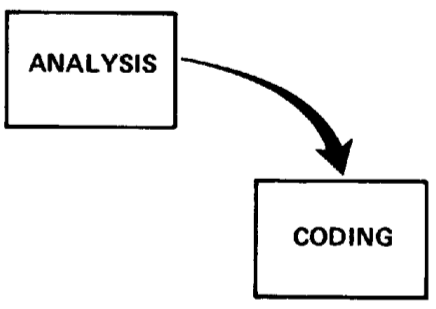
\includegraphics[width=.3\textwidth]{figures/small.png}
\alt<1>{%
	\caption{Implementación de un programa pequeño de operaciones internas}
}{}
\end{figure}

\vspace{-1em}

\alt<2>{%
Un plan para hacer sistemas más grandes que se base en estos pasos está condenado al fracaso, ya que para estos se requiere muchos otros pasos para el desarrollo de software.
}{}

\end{frame}

\section{Administración en Sistemas Grandes}

\begin{frame}[fragile]
Un mejor enfoque para proyectos grandes es usar el famoso ``diseño en cascada'', donde los pasos de análisis y código están precedidos por dos niveles de análisis de requerimientos, separados por un paso de diseño, y seguidos por un paso de testeo.

\begin{center}
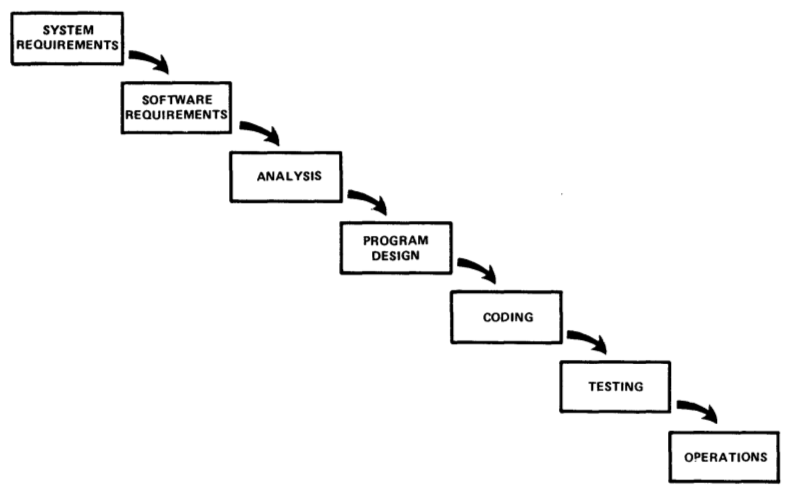
\includegraphics[height=.7\textheight]{figures/large.png}
\end{center}

\end{frame}

\begin{frame}[fragile]

Aunque este concepto es bastante bueno, la implementación es riesgosa y suele fallar.

\alt<1>{
	Idealmente, en cada paso el diseño está más detallado, y si hay un problema en alguna iteración se puede resolver en la iteración anterior.
}{}
\alt<2>{
	En el mundo real suele haber errores de diseño que no se pueden analizar precisamente hasta la fase de testing, y los cambios al diseño pueden violar los requerimientos de software y deben ser modificados.
}{}

\alt<1>{
	\begin{center}
	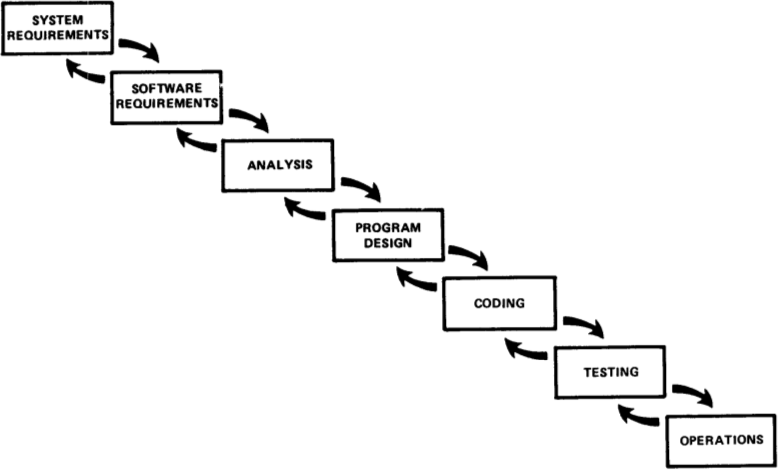
\includegraphics[height=.58\textheight]{figures/largecool.png}
	\end{center}
}{}

\alt<2>{
	\begin{center}
	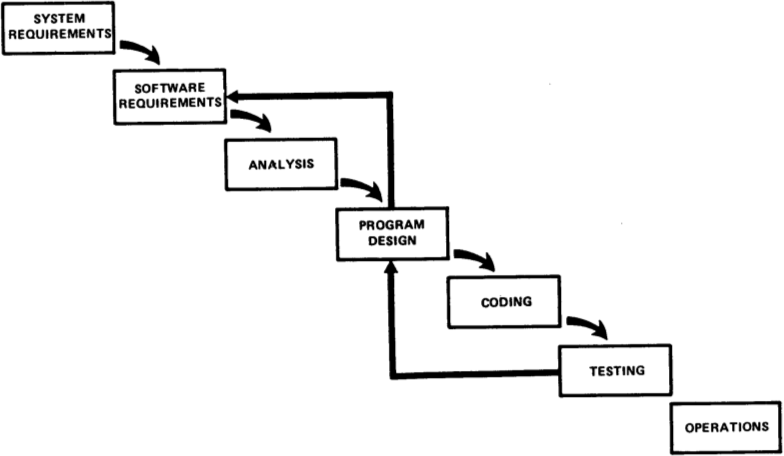
\includegraphics[height=.58\textheight]{figures/largebad.png}
	\end{center}
}{}

\end{frame}

\begin{frame}[fragile]

Sin embargo, este método sigue siendo fundamentalmente bueno. Para asegurarse que no ocurran problemas como el anterior, se pueden seguir 5 pasos que eliminan gran parte de los riesgos del desarrollo.

\end{frame}

\section{Heurísticas de Diseño}

\begin{frame}
El paper presenta 5 pasos de diseño que puede seguir el desarrollo de software para prevenir problemas como el anterior.

\begin{itemize}
\item<2-> \textbf{Program Design Comes First} (Hacer el diseño primero)
\item<3-> \textbf{Document the Design} (Documentar el diseño)
\item<4-> \textbf{Do It Twice} (Desarrollar dos veces)
\item<5-> \textbf{Plan, Control and Monitor Testing} (Planear, controlar y monitorear el testeo)
\item<6-> \textbf{Involve the Customer} (Involucrar al cliente)
\end{itemize}

\end{frame}

\subsection{Program Design Comes First}

\begin{frame}{Program Design Comes First}

Una fase de sieño preliminar se agrega entre la extraccion de requerimientos y la fase de análisis.

\centering{
\includegraphics<1>[width=.6\textwidth]{figures/design_first.png}
%\caption{Implementación de un programa pequeño de operaciones internas}
}
\begin{itemize}
\item Empezar el diseño con los diseñadores (ni analistas ni programadores)
\item Diseñar, y definir los mdoelos de procesamiento de datos.
\item Escribir un resumen entendible, informativo y actualizado.

\end{itemize}

\end{frame}

\subsection{Document The Design}


\begin{frame}{Documentar el diseño}
\frametitle{Documentar el diseño}

\begin{itemize}
\item Cuanta documentación: MUCHA
\item Más de lo que harían la mayoría de los programadores, analistas, o diseñadores por su cuenta
\item La primer regla del manejo del desarrollo de  software es la orden estricta de documetar los requerimientos.

\end{itemize}

\end{frame}


\begin{frame}{Documentar el diseño}
\frametitle{Documentar el diseño}
\begin{figure}
\includegraphics<1>[width=.5\textwidth, angle=90]{figures/design.png}
\caption{El diseño debe estar completo y ser actual}

\end{figure}


\end{frame}



\subsubsection{Hazlo dos veces}
\begin{frame}{Hazlo dos veces}

\begin{frame}{Document The Design}

\end{frame}

\subsection{Do It Twice}
\begin{frame}{Do It Twice}

Para detectar y atacar los principales riesgos tempranamente, es beneficioso implementar una corta iteración de las fases de diseño, análisis, y desarrollo obviando los detalles menos complejos.

\begin{figure}
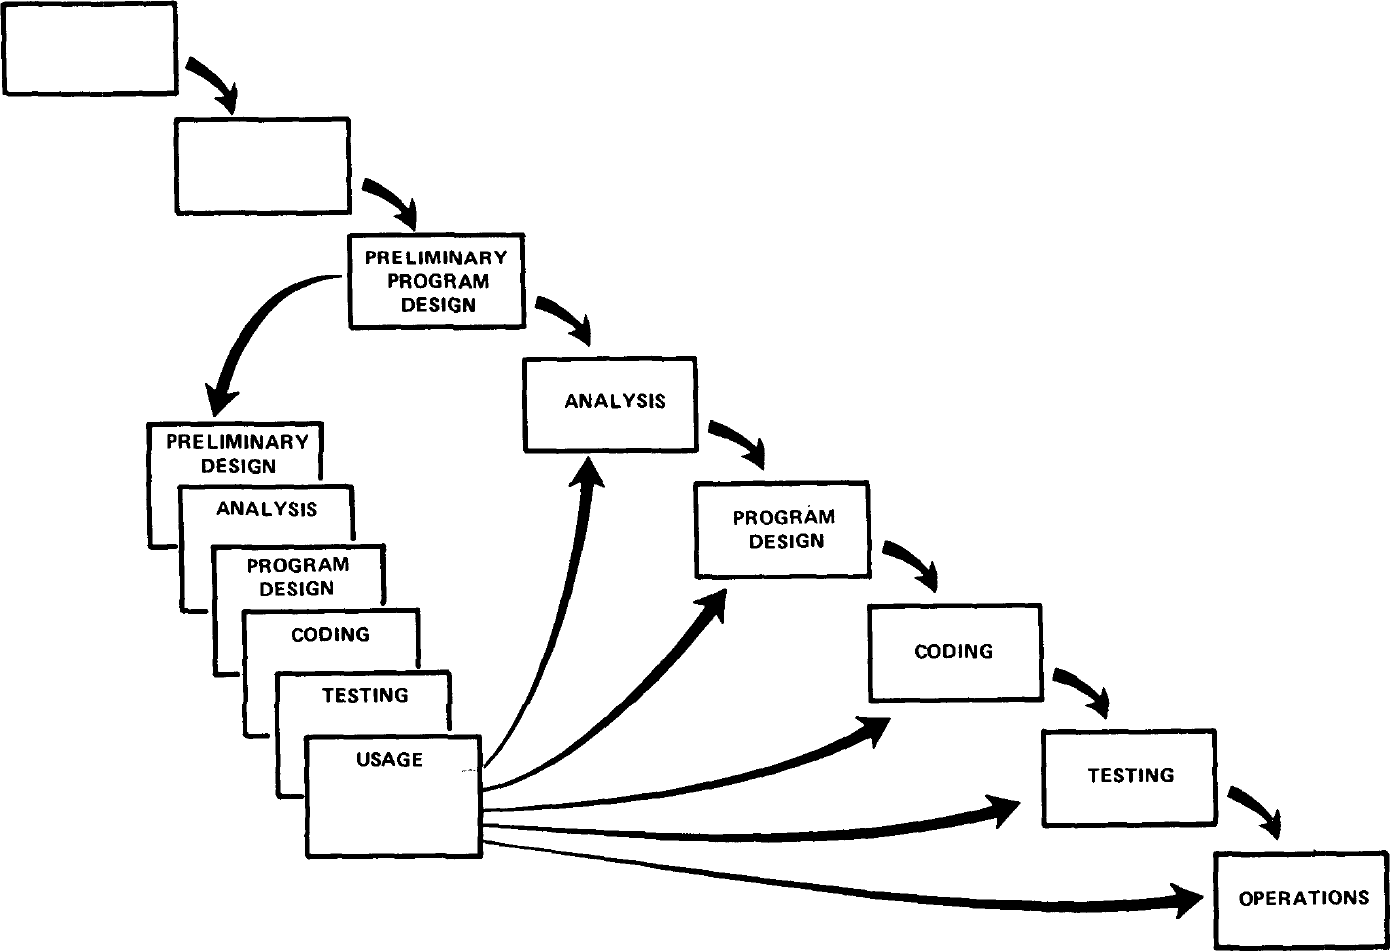
\includegraphics[width=0.5\textwidth]{figures/hazloDosVeces.png}
\end{figure}

Esto nos permite testear las hipótesis clave, para acotar el error humano en las estimaciones iniciales, que suelen ser invariablemente optimistas.

\end{frame}

\subsection{Plan, Control, and Monitor Testing}

\begin{frame}{Plan, Control, and Monitor Testing}

\end{frame}


\subsection{Involve the Customer}

\begin{frame}{Involve the Customer}

\end{frame}


\section{Bibliografía}

\begin{frame}[fragile]
\begin{thebibliography}{9}
\bibitem{royce70}
  \footnotesize
  Dr.\ Winston W.\ Royce \\
  \emph{Managing the Development of Large Software Systems} \\
  \texttt{IEEE Wescon},
  August 1970. \\
  \textit{Copyright ®1970 The Institute of Electrical and Electronics Engineers} \\
  {\scriptsize\url{https://cs.umd.edu/class/spring2003/cmsc838p/Process/waterfall.pdf}}
\end{thebibliography}
\end{frame}

\end{document}
